\section{Recurrent Neural Network for Sentiment Analysis}

\subsection{Network Architecture}
Though RNN is adapted to make use of sequential data, it is usually difficult to train the model. RNN maintains a vector of activations for each time step, which makes a RNN extremely deep~\cite{jozefowicz2015}. This also leads to the problem that it is difficult to learn long term dependencies with traditional RNN~\cite{bengio1994}. A recent summary by Pascanu et al.~\cite{pascanu2012} concluded the issues as the vanishing and the exploding gradient problems. There has been some work trying to solve the difficulty of training a RNN model. Hochreiter et al.~\cite{hochreiter1997} raised the Long Short-Term Memory (LSTM) architecture, which addresses the problem by re-parametrizing the RNN. Another model, Gated Recurrent Unit (GRU) was first presented by Cho et al.~\cite{cho2014}, is to make each unit to capture dependencies of different time scales. Chung et al.~\cite{chung2014} later evaluated LSTM and GRU on sequence modeling and found that GRU is comparable to LSTM. In our work, regarding RNN, we concentrate on LSTM.

The architecture of LSTM is shown in Figure~\ref{fig:lstm}. The first layer for LSTM is the ``forget gate layer". In this layer, the model checks $h_{t-1}$ and $x_t$, and outputs a value to represent how much information it needs to keep from previous states. 
$$f_t = \sigma (W_f \cdot [h_{t-1}, x_t] + b_f)$$
The second step consists the ``input gate layer" and a tanh layer. The ``input gate layer" is a sigmoid layer, which is used to decide what values the model needs to update. And the tanh layer creates a new vector, $\tilde{C}_t$, which could be added to current unit.
 
\begin{align*}
i_t = \sigma (W_i \cdot [h_{t-1}, x_t] + b_i) \\
\tilde{C}_t = tanh(W_c \cdot [h_{t-1}, x_t] + b_C)
\end{align*}

And next, the model will obtain $C_t$ from multiplying old state by $f_i$, multiplying $\tilde{C}_t$ by $i_t$ and summing them up. 
$$C_t = f_t * C_{t-1} + i_t * \tilde{C}_t$$
Finally, the model needs to decide the output. The output gate layer implements operations on $C_t$ and $o_t$, and output $h_t$ for the next state.

\begin{align*}
o_t = \sigma (W_o [h_{t-1}, x_t] + b_o) \\
h_t = o_t * tanh(C_t)
\end{align*}

\begin{figure}
\centering
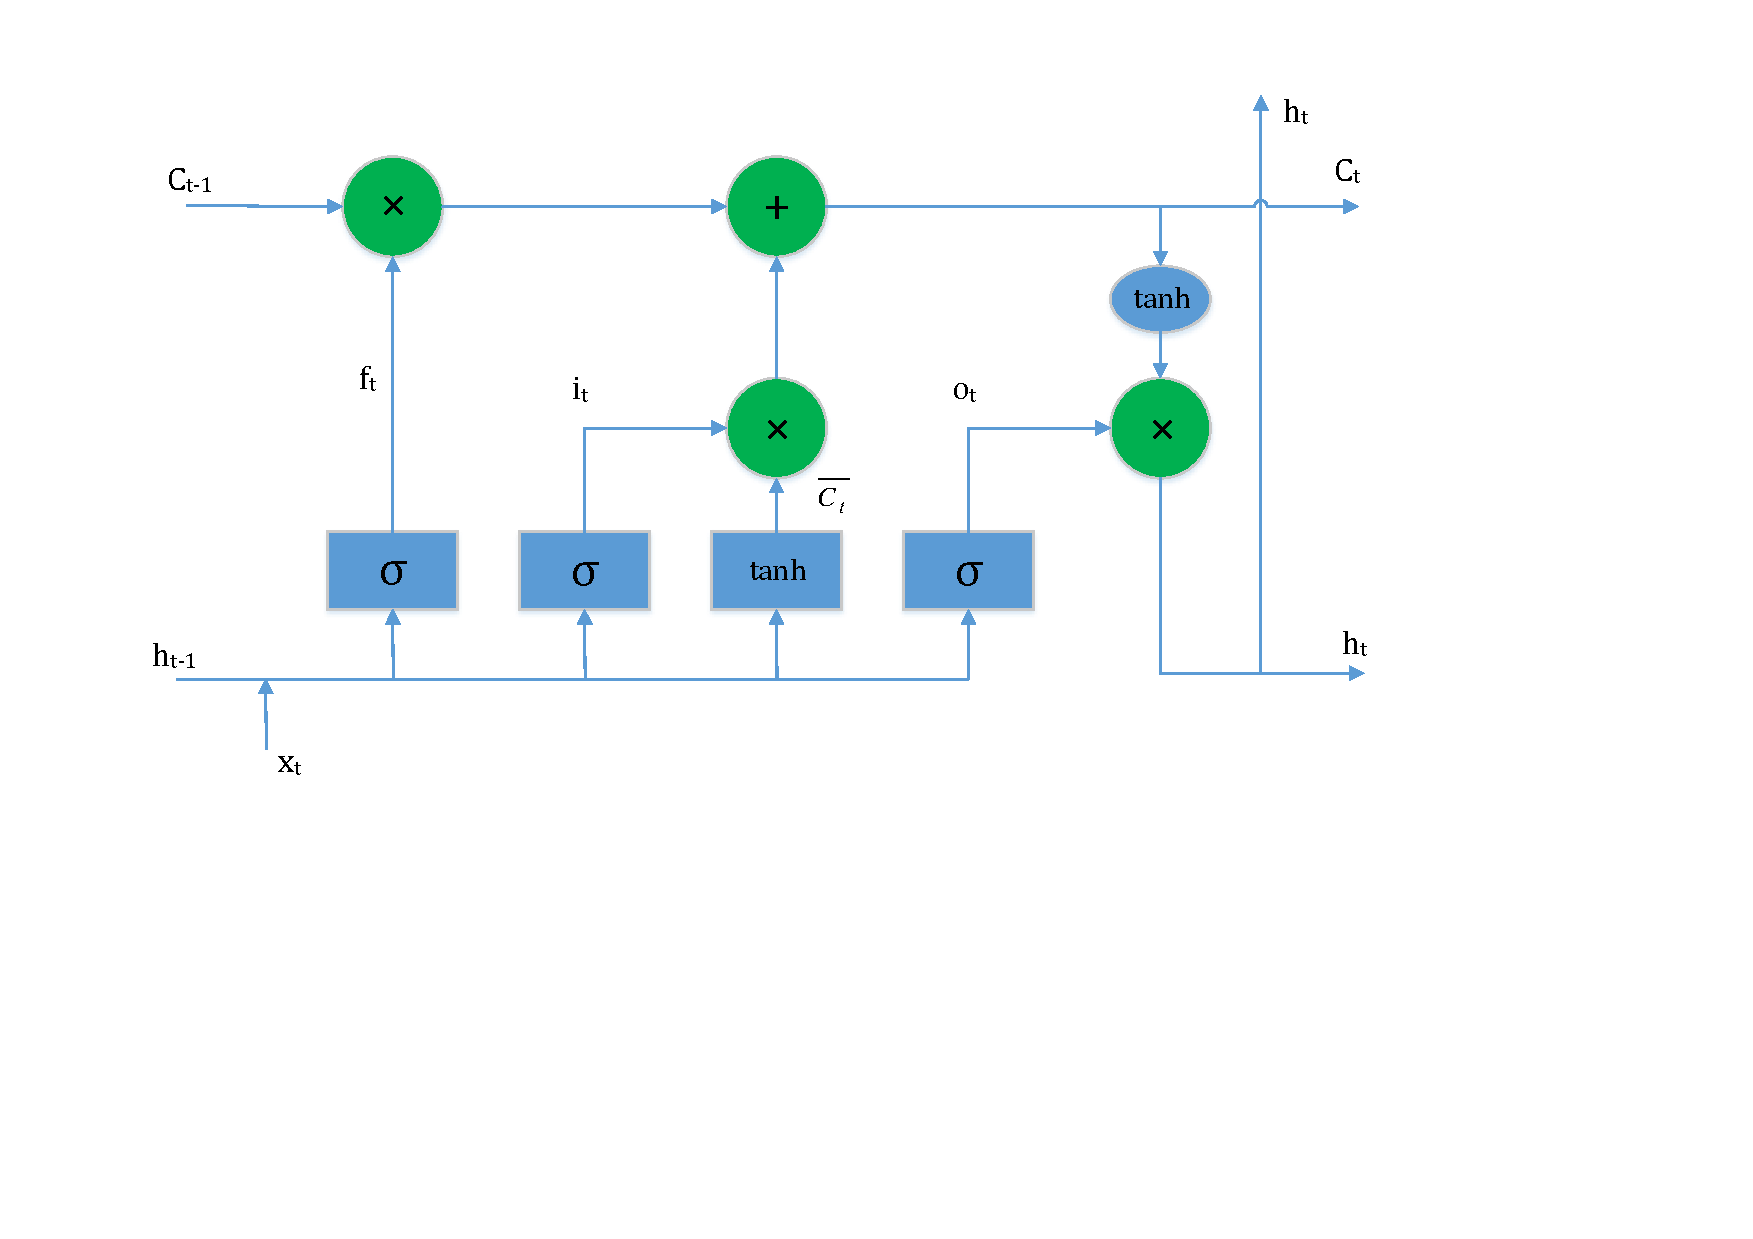
\includegraphics[scale=0.6]{figure/lstm.pdf}
\caption{Architecture of Long Short-Term Memory.}
\label{fig:lstm}
\end{figure}

\begin{figure}
\centering
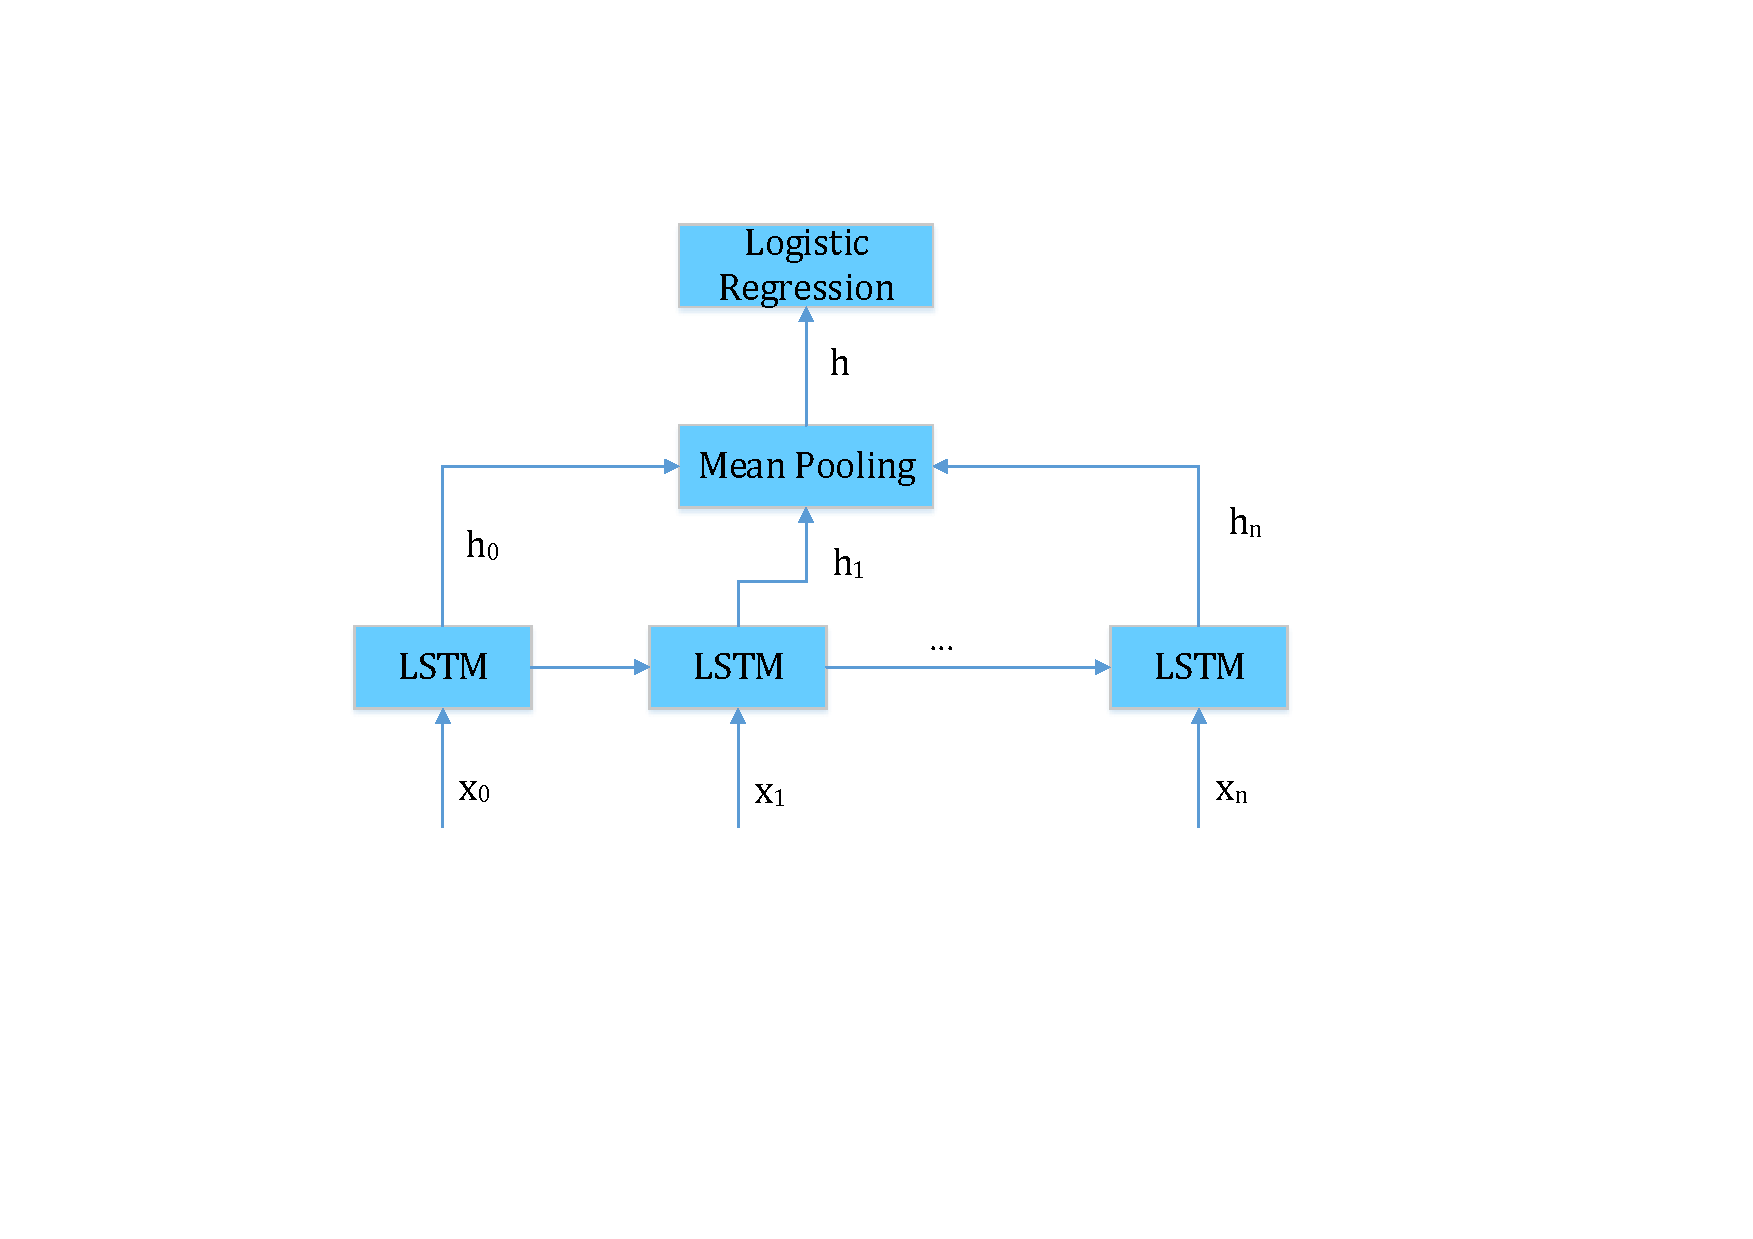
\includegraphics[scale=0.6]{figure/lstm_model.pdf}
\caption{LSTM model used in our report.}
\label{fig:lstm_model}
\end{figure}

The deep learning model we use in the report is a variance of classical LSTM. And the structure of the LSTM variance is shown in Figure~\ref{fig:lstm_model}. In our model, the output of current state does not depend on current memory cell state $C_t$, but just on input $x_t$ and $h_{t-1}$. So, the equation of $o_t$ is updated to
$$
o_t = \sigma (W_o x_t + U_o h_{t-1} + b_o)
$$

Additionally, the model also consists of a mean pooling layer and a logistic regression layer. For every LSTM cell, it outputs information $h_i$. And by averaging all of the output sequence, mean pooling outputs $h$ and it is fed to the logistic regression layer. Then the logistic regression layer will train the model according to class labels and associated sequences.

\subsection{Experiment}
For the LSTM model for sentiment analysis, we design and evaluate the model on two different kinds of sentiment data sets. The first one is the Stanford Twitter corpus, which has been described in previous section. And the second data set is the Large Movie Review Dataset~\cite{maas2011}, which consists of 25,000 highly polar movie reviews for training, and 25,000 reviews for testing. In the 25,000 training reviews, there are 12,500 positive reviews and 12,500 negative reviews.

During the pre-processing step, we utilize the count-based method to represent the words in the data sets. A count-based approach takes advantage of the assumption that words which have similar counts in a text context, share similar semantic meaning. This approach is opposite to context-predicting semantic vectors such as {\tt word2vec} which is used in our experiment of CNN. The difference between the two word representation models were discussed in~cite{baroni2014}. 

The LSTM model is implemented in Theano~\cite{bastien2012, bergstra2010}, which is a Python library for deep learning. It allows users to define, optimize and evaluate mathematical expression efficiently and conveniently. 

We run the LSTM model on each of the two data sets three times, and calculate the mean value of the accuracies. While, we observe a dramatic difference between the two data sets. The accuracy of Stanford Twitter corpus is as low as 54.6\%, but the accuracy of IMDB dataset is as high as 81.7\%. To explain the large gap between the results, we think there may be following reasons:

\begin{enumerate}
\item The paramters of the LSTM model on Stanford Twitter corpus needs to tuned. Even though we have adjusted the parameters for every specific dataset, we did not find the best settings for Twitter sentiment analysis.
\item LSTM is good at capturing long time dependency information in a corpus. While, for tweets, actually, they are usually very short, and there is little dependency information existed. Our LSTM model may not fit well in this case.
\end{enumerate}




